\section{Improving HuMoR TestOps}
\label{sec:humor_improvement}

This section presents the attempt that was made at modify the TestOps of the HuMoR paper \cite{humor} in such a way that we attain comparable results but in a significantly shorter timespan.

\TODO{See if I have introduced the terms properly (decoded sequence, $x$'s, $x'$'s, etc.)}

\subsection{Speeding up the TestOps}

Realising that the main speed limitations are due to the concept of rollout over the entire sequence, we decided to break this long range dependence. Through short overlapping rollouts, it is possible to acheive more parrallelisation and smaller computation graphs, and our intuition suggests that the need for such a large context window is not necessary, that only a small number of autoregressed frames are needed to be able to propagate information sensibly and to get meaningful gradients. Anecdotaly, it would seem intuitive that if a video contains sitting, then walking, then sitting again, the second act of sitting would not depend in on the early act of sitting, hence rolling out over the whole sequence seems unnecessary.

The HuMoR TestOps rollout is presented graphically in \figref{fig:humor_rollout_graph}. $x$ is the state, and $z$ are the latent variables, the optimised variabels are highlighted in pink, and the losses are coloured, gray x's indicate they are calculated during the optimisation from the optimised variables. As can be seen, first all the states are autoregressed from the initial state and the latent variables, and then the losses are applied. This can be seen to result in very long range dependencies in the computation graph, thus making the gradients time consuming to calculate. 

\begin{figure}[h!]
    \centering
    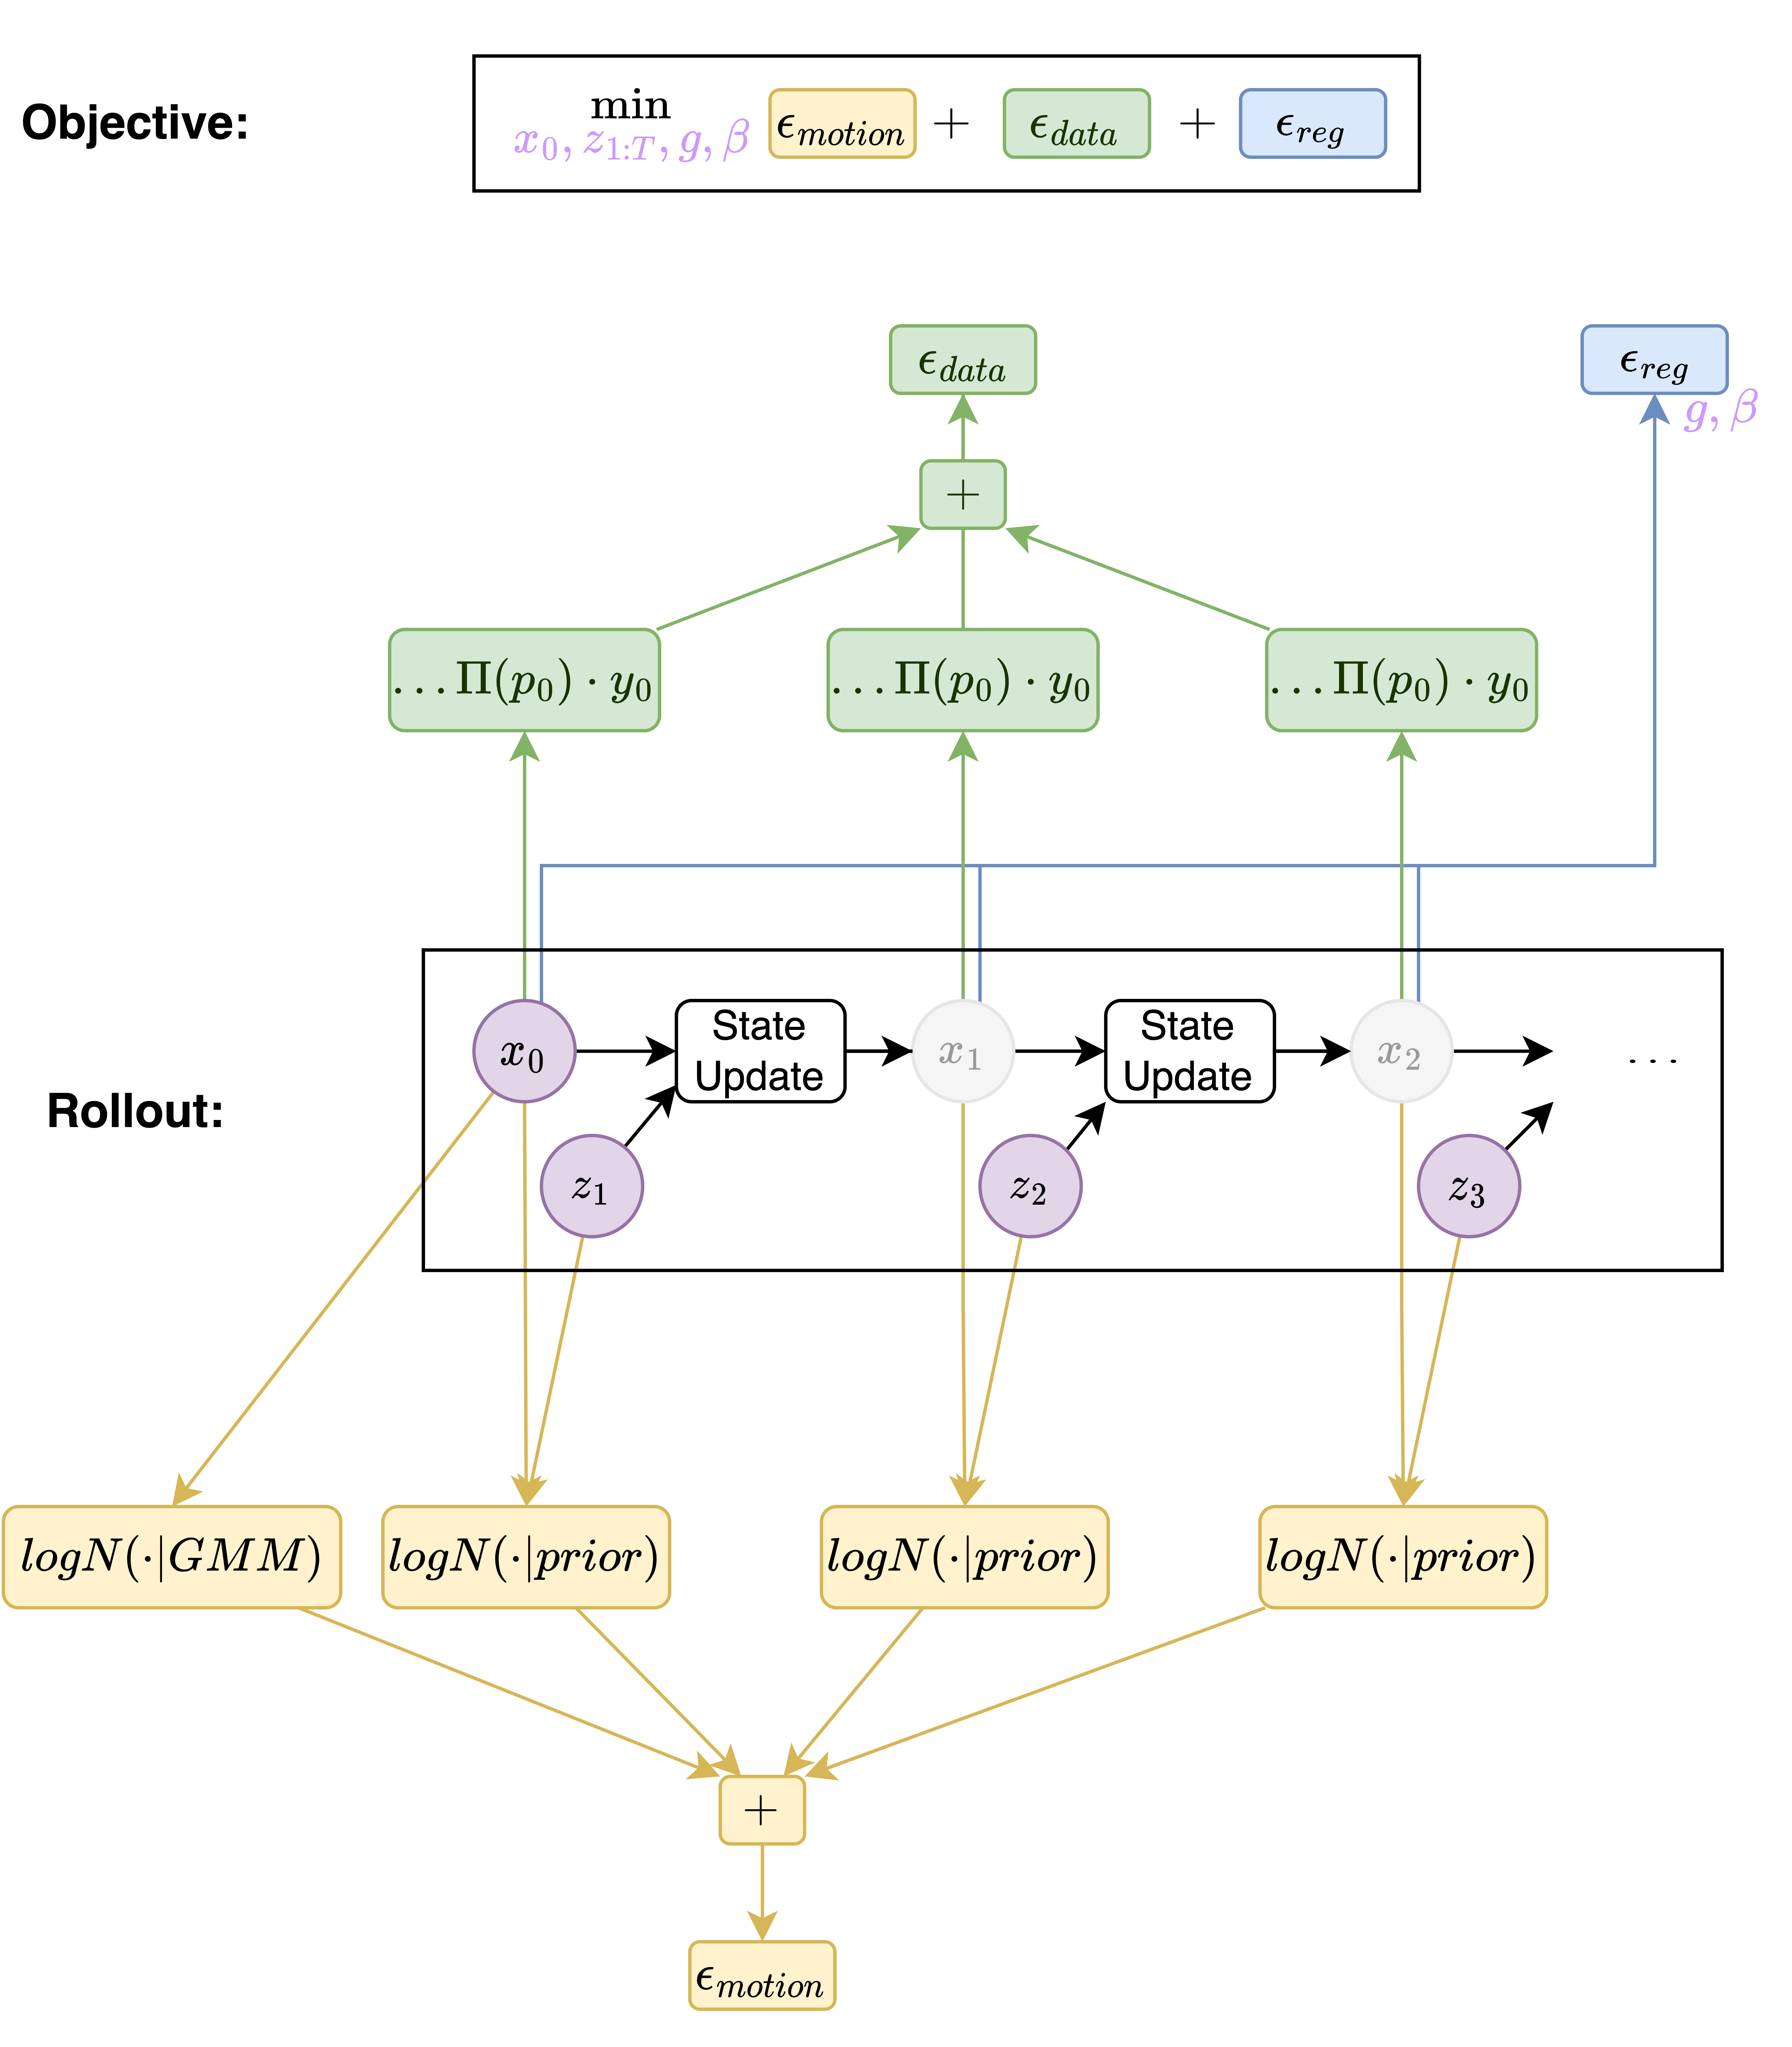
\includegraphics[width=1\textwidth]{Figures/humor/improvement/computation_graph_humor.png}
    \caption{TestOps Computation Graph}
    \label{fig:humor_rollout_graph}
\end{figure}

\TODO{Update \figref{fig:dimm_rollout_graph} and remove the 'NEW' norm, labels on green loss, and potentially red loss?}

The most obvious way to break this autogregression is to maintain and optimise a separate sequence of $x$'s, updating this seperate sequence with reference to the $x'$'s decoded from the latent variables as in \figref{fig:dimm_rollout_graph}. We can take into account the decoded $x'$'s in several manners:
\begin{itemize}
    \item Copy over
    \begin{itemize}
        \item Directly replace the optimised sequence of $x$'s with the decoded $x'$'s.
    \end{itemize}
    \item Blend
    \begin{itemize}
        \item Perform a weighted addition of the optimised $x$'s and decoded $x'$'s.
    \end{itemize}
    \item Loss term
    \begin{itemize}
        \item Add a loss term on the difference between the optimised $x$'s and decoded $x'$'s. 
    \end{itemize}
\end{itemize}

All decoding steps can now be performed in parrallel, rather than sequentially, which greatly reduces the computation time. 

\begin{figure}[h!]
    \centering
    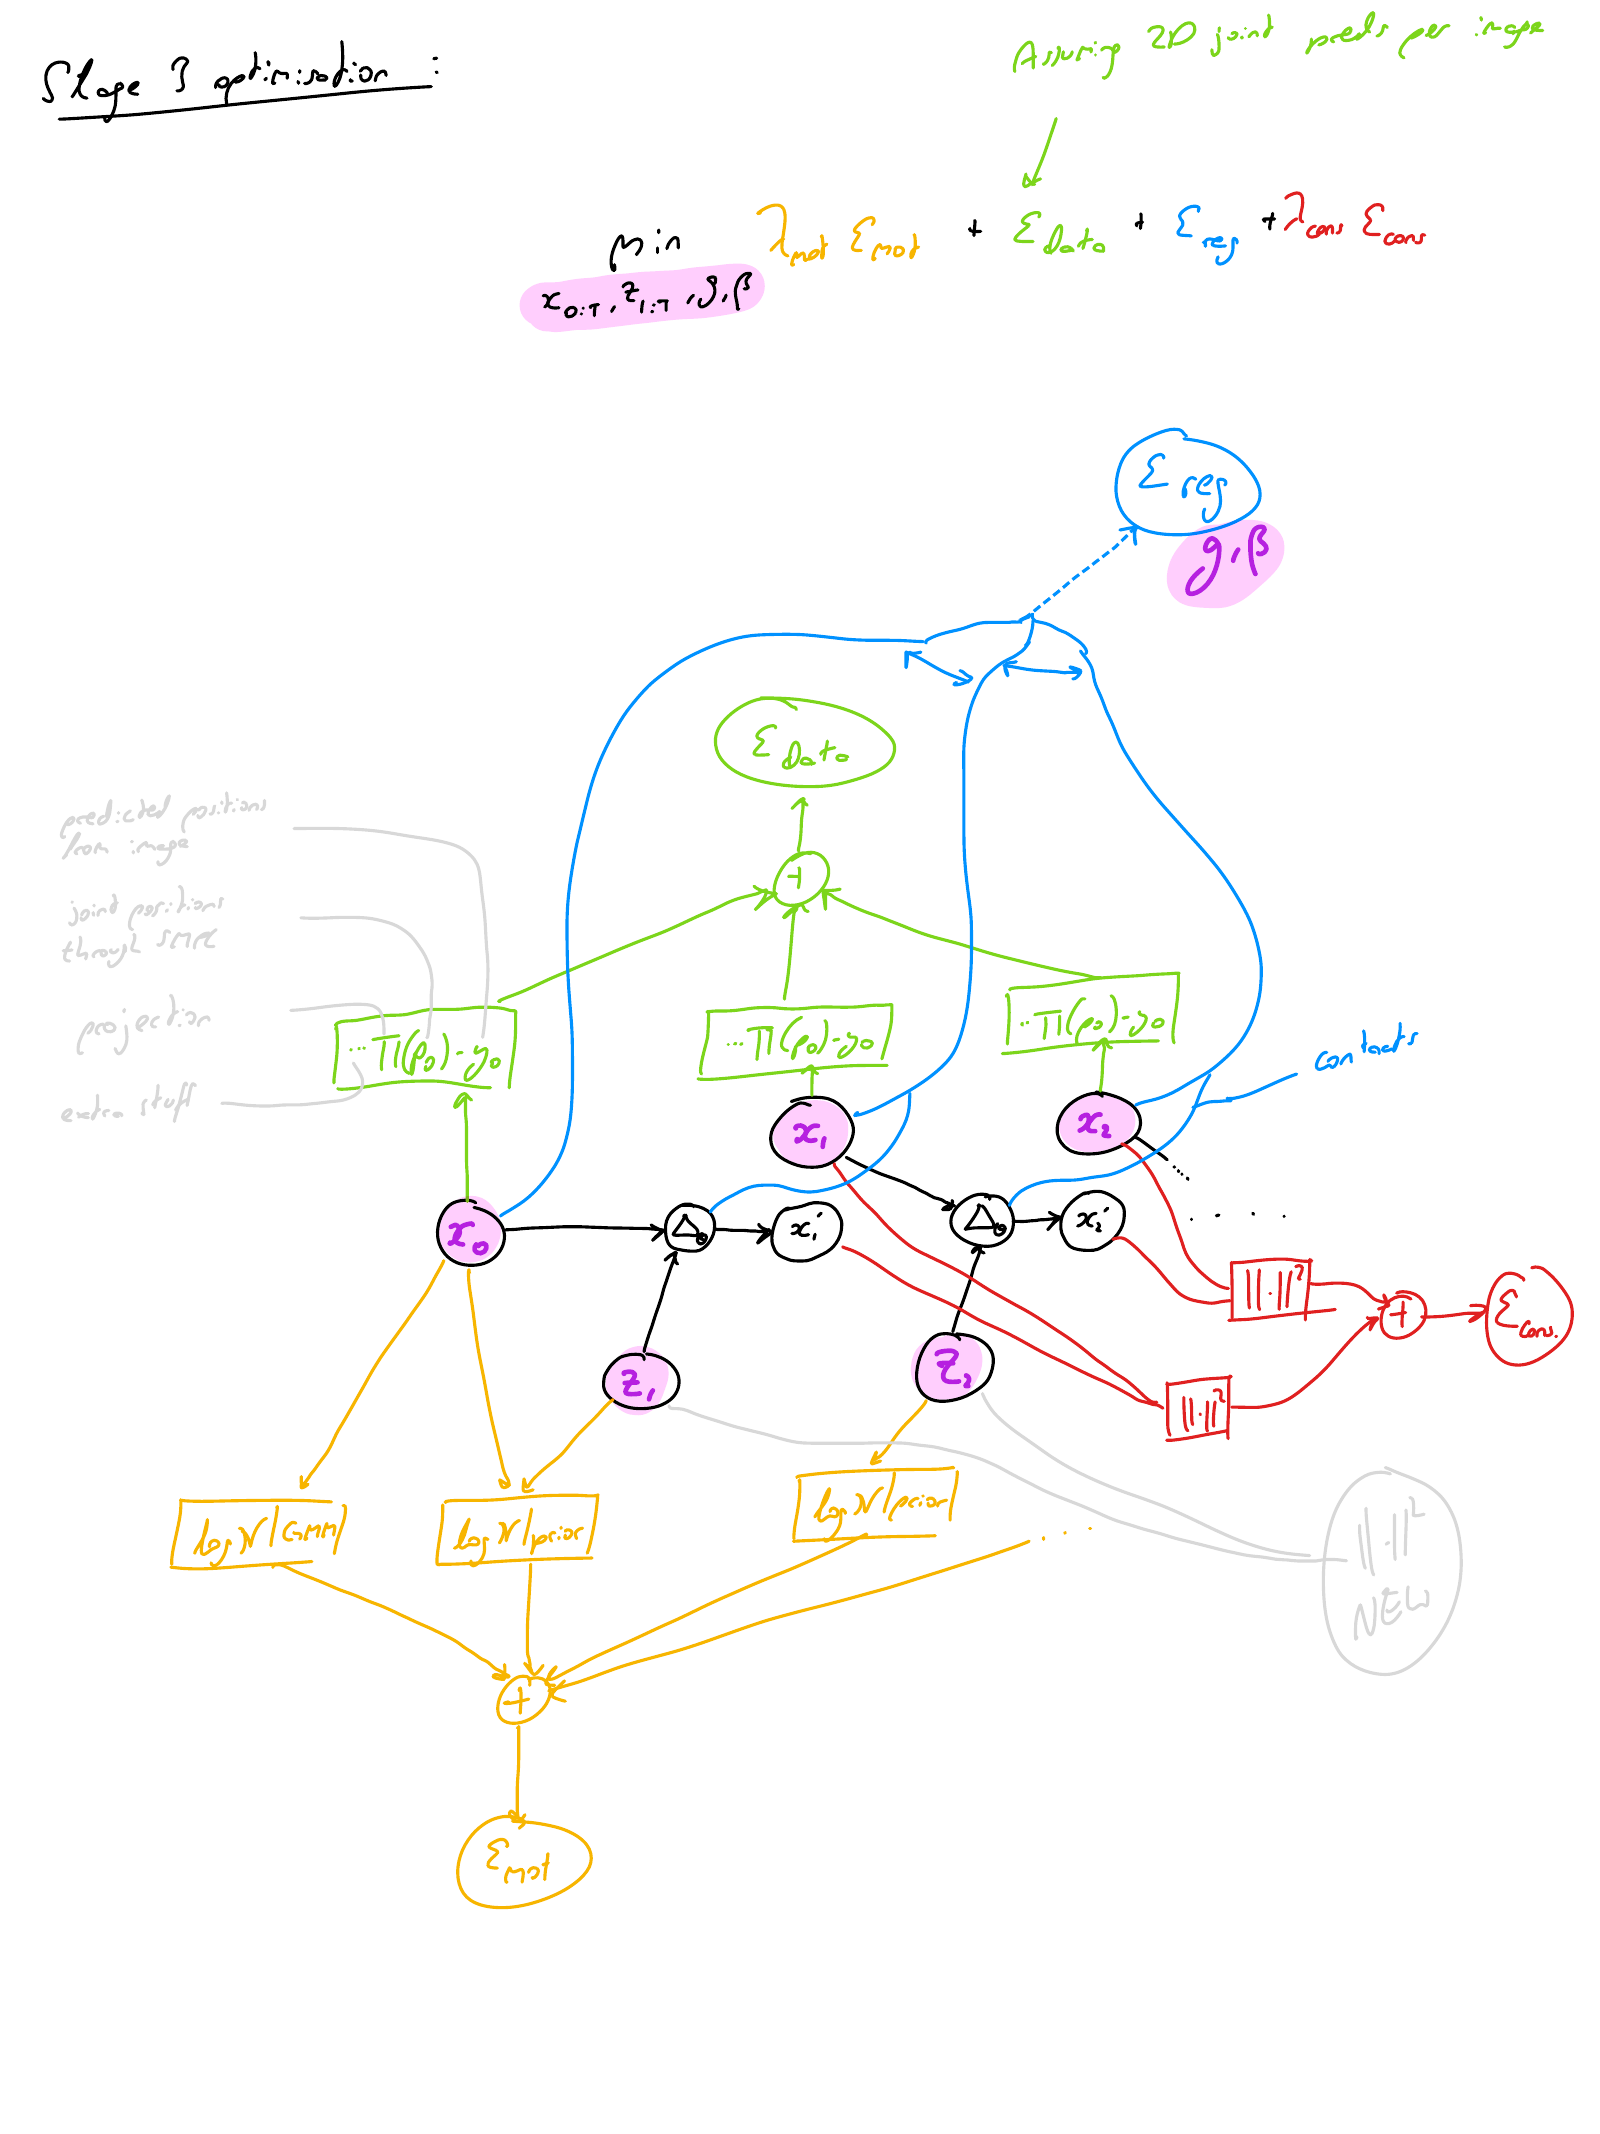
\includegraphics[width=1\textwidth]{Figures/humor/improvement/computation_graph_dimm.png}
    \caption{Decoupled Computation Graph}
    \label{fig:dimm_rollout_graph}
\end{figure}

This new method also allows us to experiment with different amounts of rollout. We can once again decode the decoded sequence of $x'$'s to get $x''$, and so on and so forth. These extra sequences are all decoded with the same latent variables thus the updates to the latent variables will take into account the losses on all the decoded sequences. Graphically this can be seen in \figref{fig:dimm_decoded_sequences}, where each next line .
\TODO{describe the figure better}

\begin{figure}[h!]
    \centering
    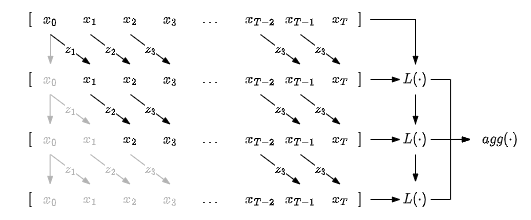
\includegraphics[width=1\textwidth]{Figures/humor/improvement/Rollout_overlap.png}
    \caption{Decoded sequences}
    \label{fig:dimm_decoded_sequences}
\end{figure}

The information contained in each $x$ can flow forwards through the short range rollouts, and over the iterations of the optimiser. Note however that the information flow will be slower than the HuMoR TestOps, as in the TestOps all subsequent $x$'s are regressed from the initial $x_0$.
In the HuMoR TestOps information can flow backwards from any future frame's $x$ in one update through the gradients, as all $x$'s are linked in the computation graph through the auto-regression (though our intuition suggests that the information does not actually need to flow so far, as previously discussed). In the new method however, the information flow will be much more limited, as the rollouts will be significantly shorter, though again the information should flow through the iterations fo the optimiser.

\subsection{Implementation notes}

A number of issues were encountered during the implementation that are worth mentioning. After implementing the new method, attempts were made to get the optimiser to produce sensible results. The general approach was to use a small number of losses, so as to get a better intuition of each loss, with the goal of better understanding how to balance the losses in the optimiser, but some errors in individual losses were encountered.

Firstly, as expected, the Axis-Angle representation became a problem. When running through functions to convert to root-local reference frame for the HuMoR model for decoding (as it operates on said reference frame), and then back to world reference frame for the opftimiser, the Axis-Angle vector flipped direction. Though the flipped vector still represented the same rotation, the angle representations of the same angle in the optimised sequence of $x$'s and the decoded sequence of $x'$'s were different, hence encorporating the information from decoded sequence cause the angle to move somewhere between the two flipped values which was no longer a sensible angle representation, thus resulting in root flips and other strange effects.

Secondly, an issue due to the SMPL model was found. When using a 2d reprojection loss (comparing the projected SMPL joints to the OpenPose 2d predictions) on a sequence where only the left arm and face had any OpenPose predictions, the legs were being moved by the optimiser. This was wrong as there were only losses on the arm and face joints, hence no gradients should flow to the legs. It was eventually found that the skinning weights of the SMPL model \cite{SMPL} contain spurious long range connections. 3\% of the LBS (linear blend skinning) weights in the SMPL model are non-zero but less than $1e-2$, which seems rather too low to have any meaningful effect on the skinning, but which allows for spurious gradients to flow. \\
For the comparison to the OpenPose predictions the OpenPose skeleton must be obtained from the SMPL mesh. Certain joints are regressed, other are simply taken directly as vertices from the mesh, as in the case of the nose joint in the OpenPose skeleton which is taken to be vertex 332 \cite{SMPL_op_joints}. We noted that this vertex 332 is skinned $99.8\%$ by the 'head' joint, but also $0.2\%$ by the right hip, left knee and right knee. This issue was solved by pruning all weights below 1e-2. It is interesting to note that there are known spurious connections in the SMPL blend shapes \cite{STAR}, but that we have found no reference to spurious connections in the LBS weights.

\subsection{Experiments}

% c.f Current_experiments.md for more details
\TODO{explain why the initial rollout was bad, and the compounding of errors forward}
\TODO{maybe we should discuss more in the humor investagtion section about the bad initial rollout}
\TODO{Check everything is explicitely named, e.g have a graphic clearly naming the optimised x's and the decoded x's, and what the z's are}

To begin with, we looked into the initial $z$'s that were obtained from projecting the Stage 2 results through the HuMoR encoder. We found that in occluded situations these $z$'s encode a sitting motion without any optimisation as seen in \figref{fig:humor_stage_2_rollout_sitting}, that simply the projection leads them to encode the necessary occluded motion. However we note that when autoregressively rolled out over a longer sequence the results, in \figref{fig:humor_stage_2_rollout_deviation}, deviate largely from the initial sequence of $x$'s seen in \figref{fig:humor_stage_2}. This shows us that though the initial $z$'s encode some sensible motion locally, and can be used to accurately recover the next frame, when they are chained together small deviations from the $x$ motion accumulate to create an overall deviation. For example if the arm is moved slightly too much by a single $z$, then all the future frames will have the arm in slightly the wrong position, and multiple $z$'s are wrong in the same direction, then the arm will raise up. This deviating sequence is the initial starting rollout in the Stage 3 of the HuMoR TestOps in which the rollout is optimised, though it seems unfortunate to us that from a sensible sequence of $x$'s obtained from Stage 2 we get such a bad sequence through the autoreggresive rollout. We do however note that though while this starting point represents a sequence that deviates largely, the $z$'s might not need to move so far to avoid the accumulation effect. The intuition in our case was that we are starting from some sensible $x$'s and $z$'s, and therefore that it should be possible to refine the $x$'s by take into account the HuMoR model through the $z$'s whilst updating the $z$'s. 

\begin{figure}[h!]
    \centering
    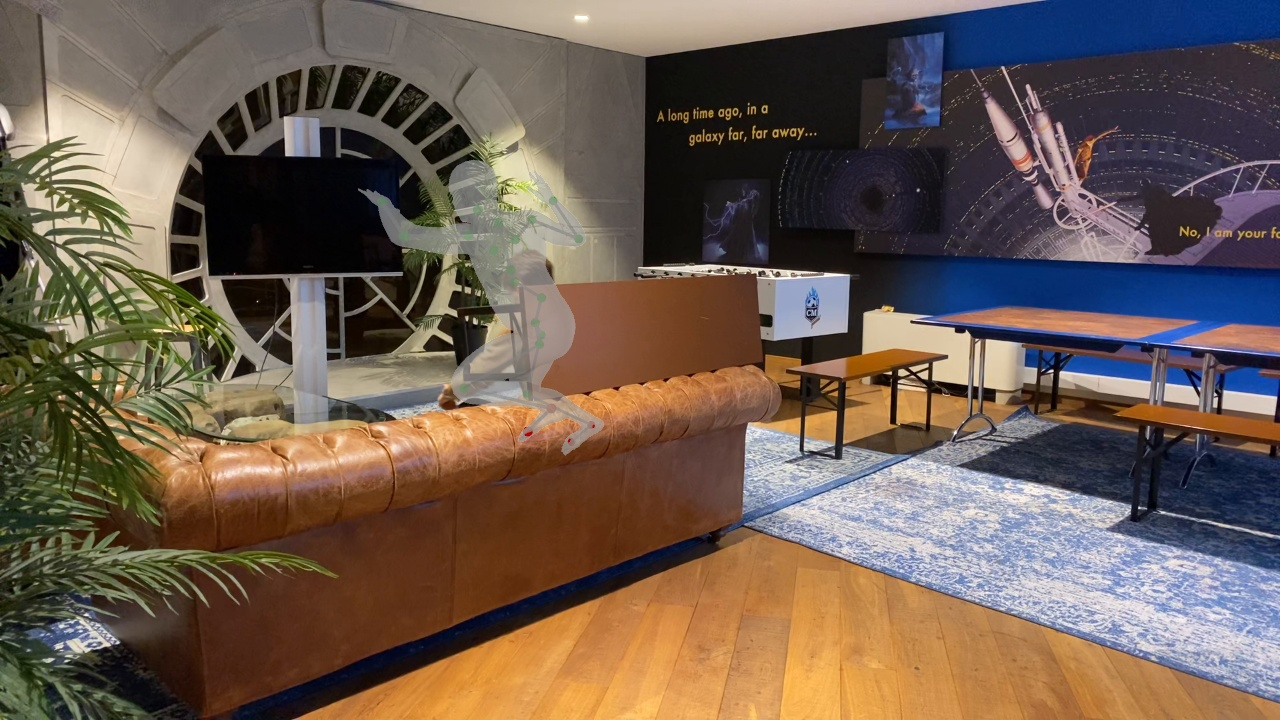
\includegraphics[width=1\textwidth]{Figures/humor/improvement/Rollout_stage_2/sitting_clip/rollout_sitting_example/frame_00000078.jpg}
    \caption{Stage2 $z$'s encode a sitting motion}
    \label{fig:humor_stage_2_rollout_sitting}
\end{figure}


\begin{figure}[h!]
    \centering
    \subfloat[]{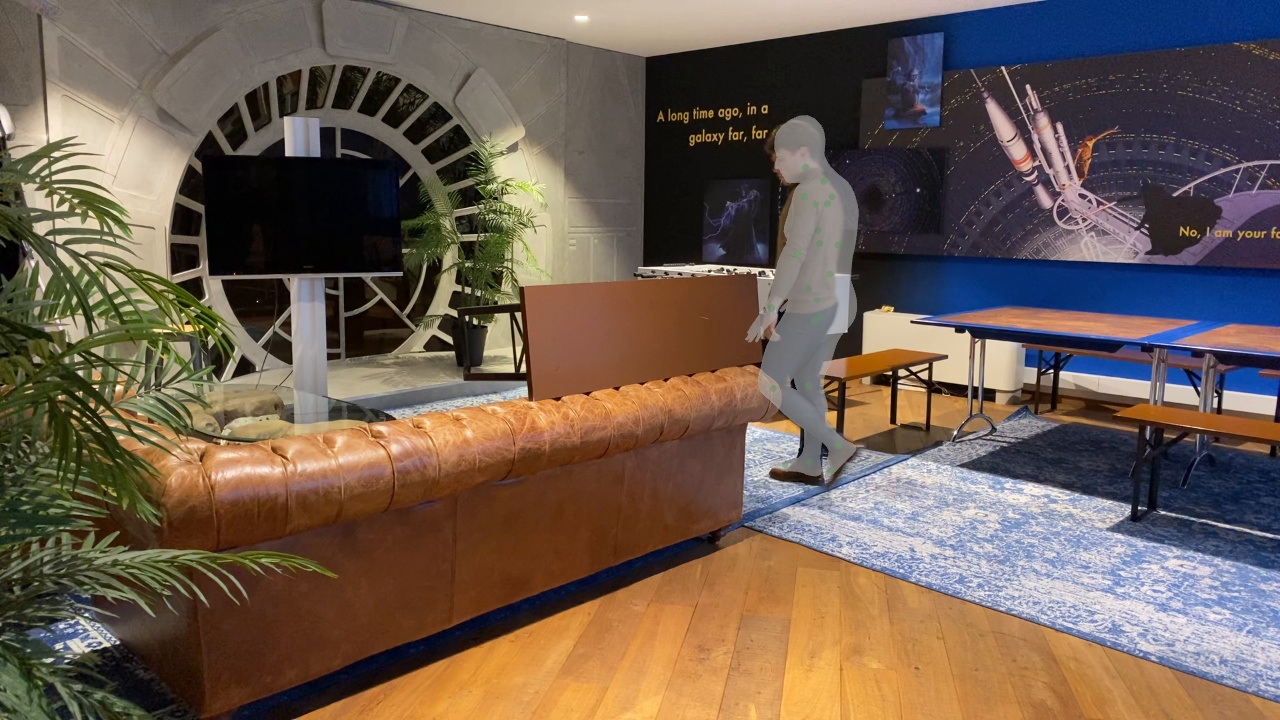
\includegraphics[width=0.3\textwidth]{Figures/humor/improvement/Rollout_stage_2/sitting_clip/stage2/frame_00000099.jpg}} 
    \hfil
    \subfloat[]{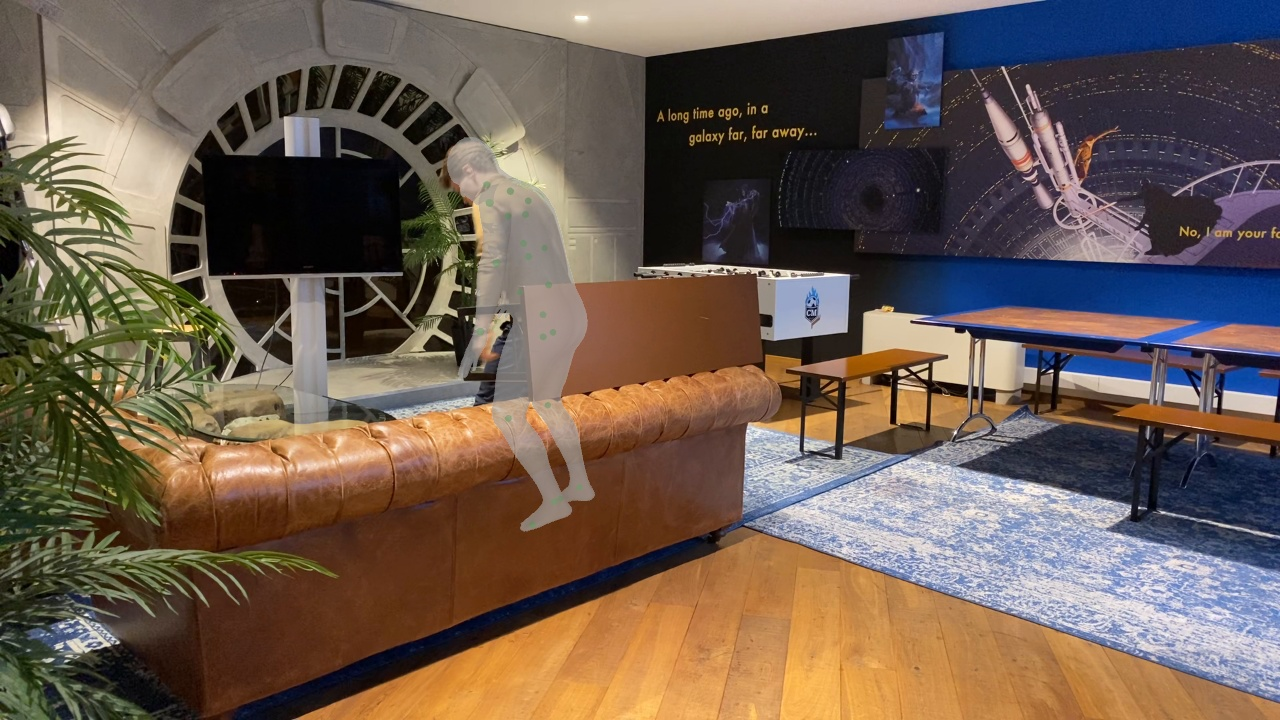
\includegraphics[width=0.3\textwidth]{Figures/humor/improvement/Rollout_stage_2/sitting_clip/stage2/frame_00000149.jpg}} 
    \hfil
    \subfloat[]{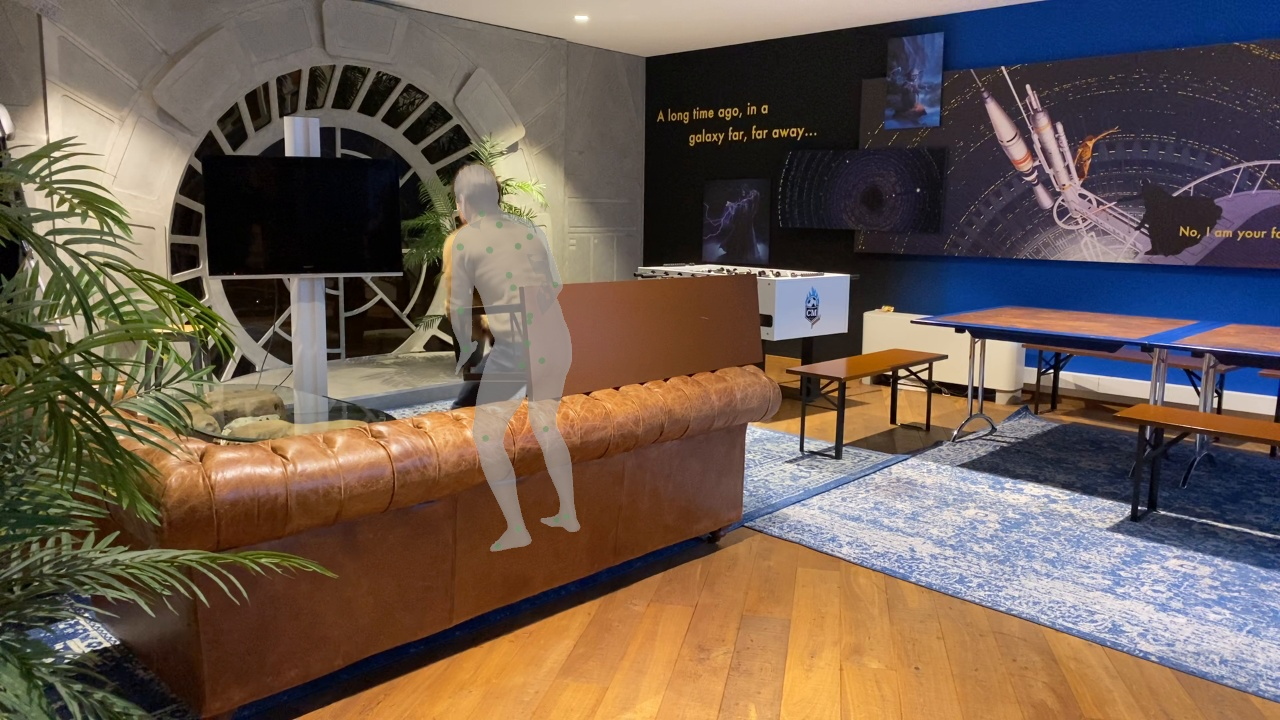
\includegraphics[width=0.3\textwidth]{Figures/humor/improvement/Rollout_stage_2/sitting_clip/stage2/frame_00000219.jpg}}
    \hfil
    \subfloat[]{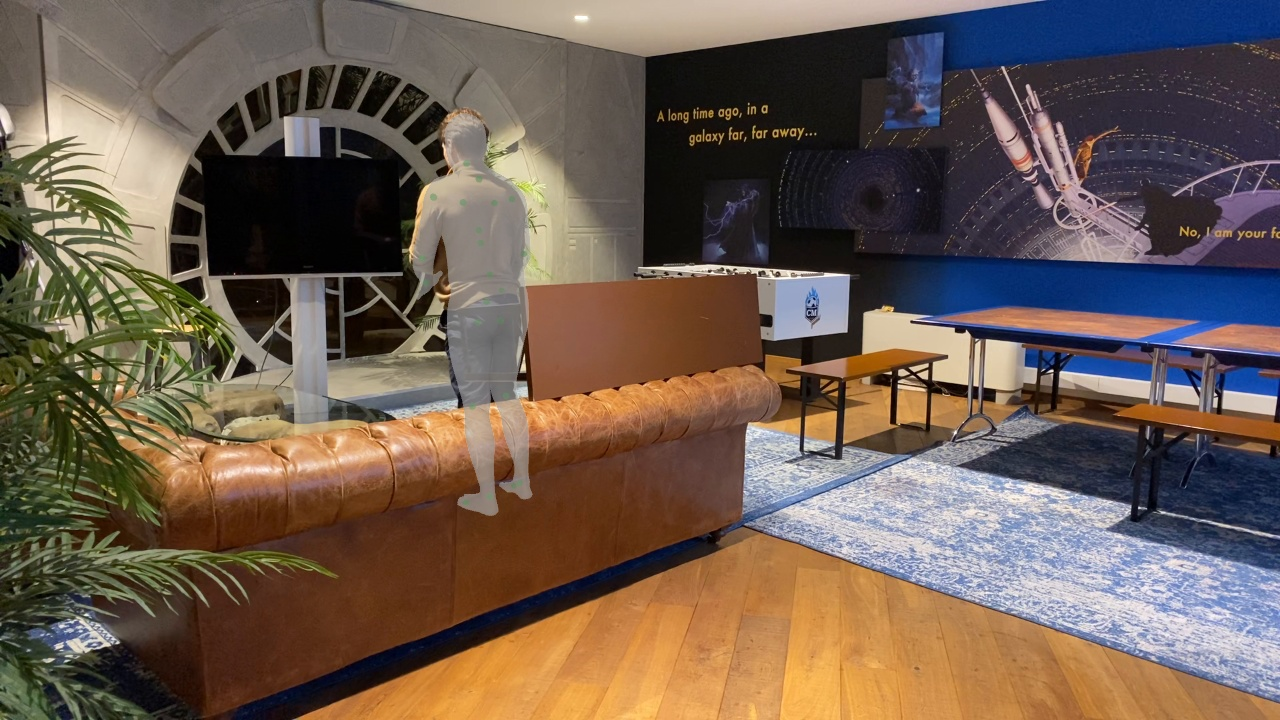
\includegraphics[width=0.3\textwidth]{Figures/humor/improvement/Rollout_stage_2/sitting_clip/stage2/frame_00000239.jpg}}
    \caption{Stage 2 $x$'s}
    \label{fig:humor_stage_2}
\end{figure}

\begin{figure}[h!]
    \centering
    \subfloat[]{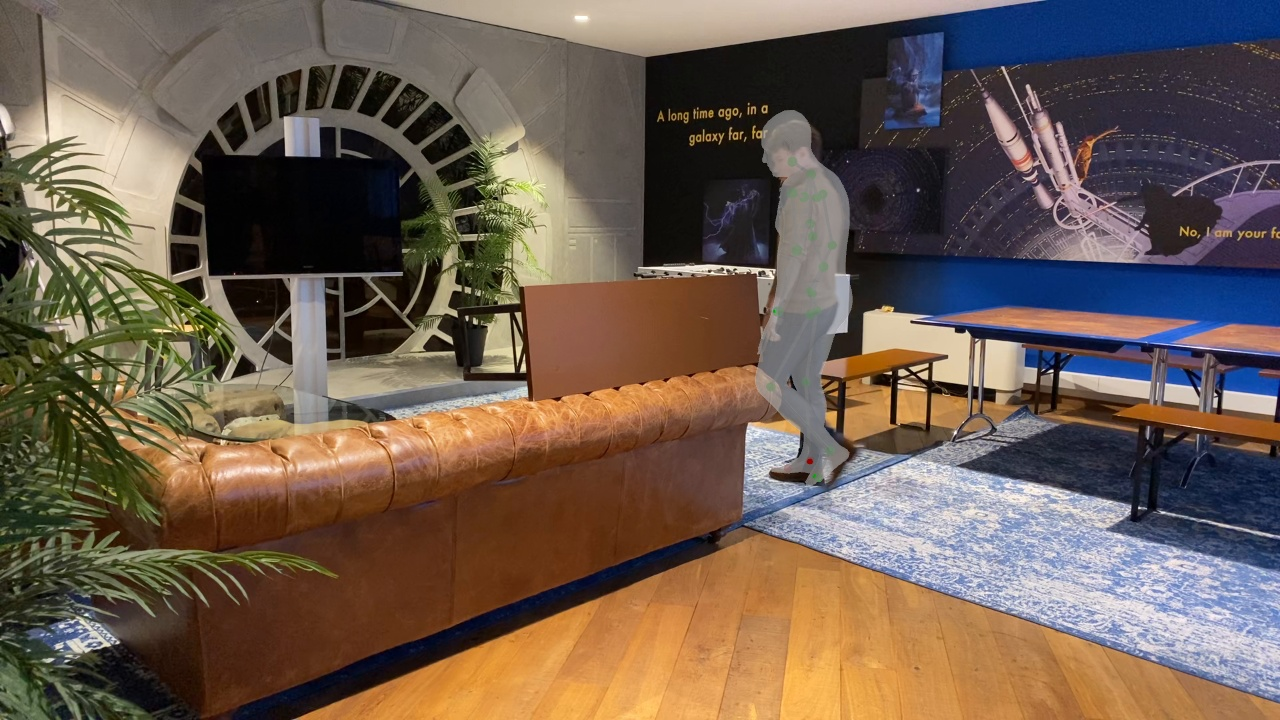
\includegraphics[width=0.3\textwidth]{Figures/humor/improvement/Rollout_stage_2/sitting_clip/rollout/frame_00000010.jpg}} 
    \hfil
    \subfloat[]{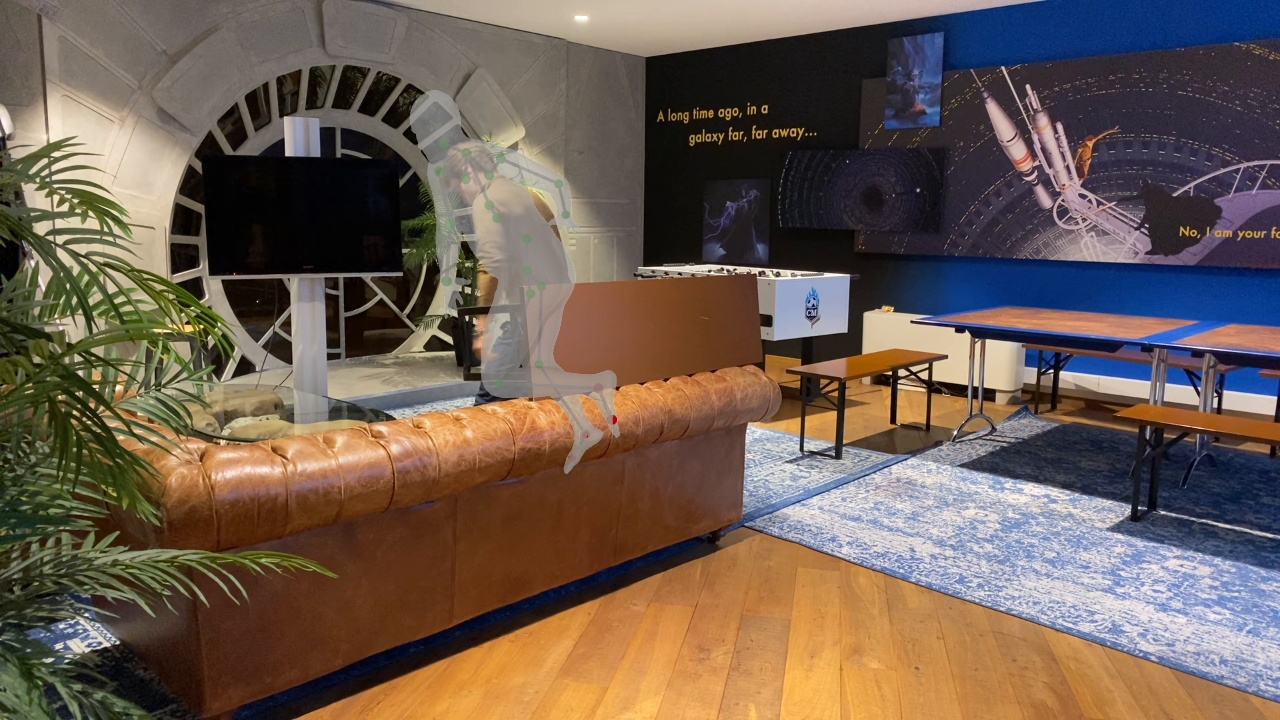
\includegraphics[width=0.3\textwidth]{Figures/humor/improvement/Rollout_stage_2/sitting_clip/rollout/frame_00000060.jpg}} 
    \hfil
    \subfloat[]{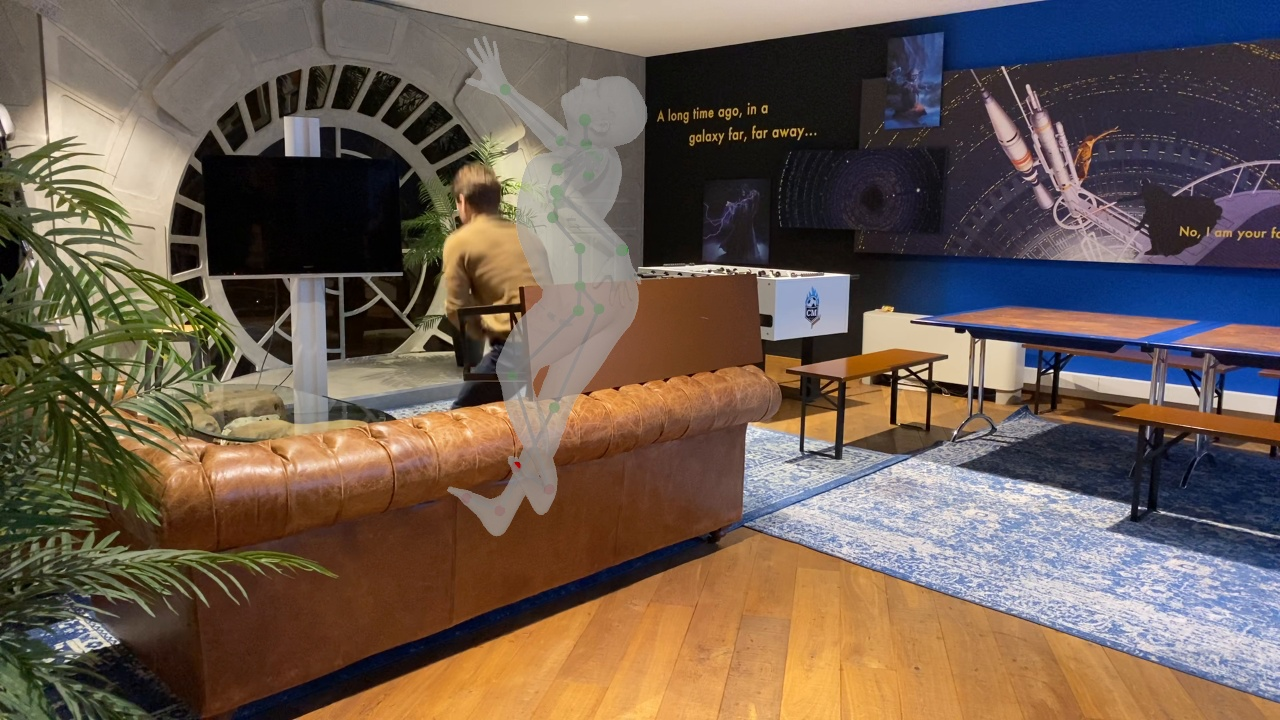
\includegraphics[width=0.3\textwidth]{Figures/humor/improvement/Rollout_stage_2/sitting_clip/rollout/frame_00000130.jpg}}
    \hfil
    \subfloat[]{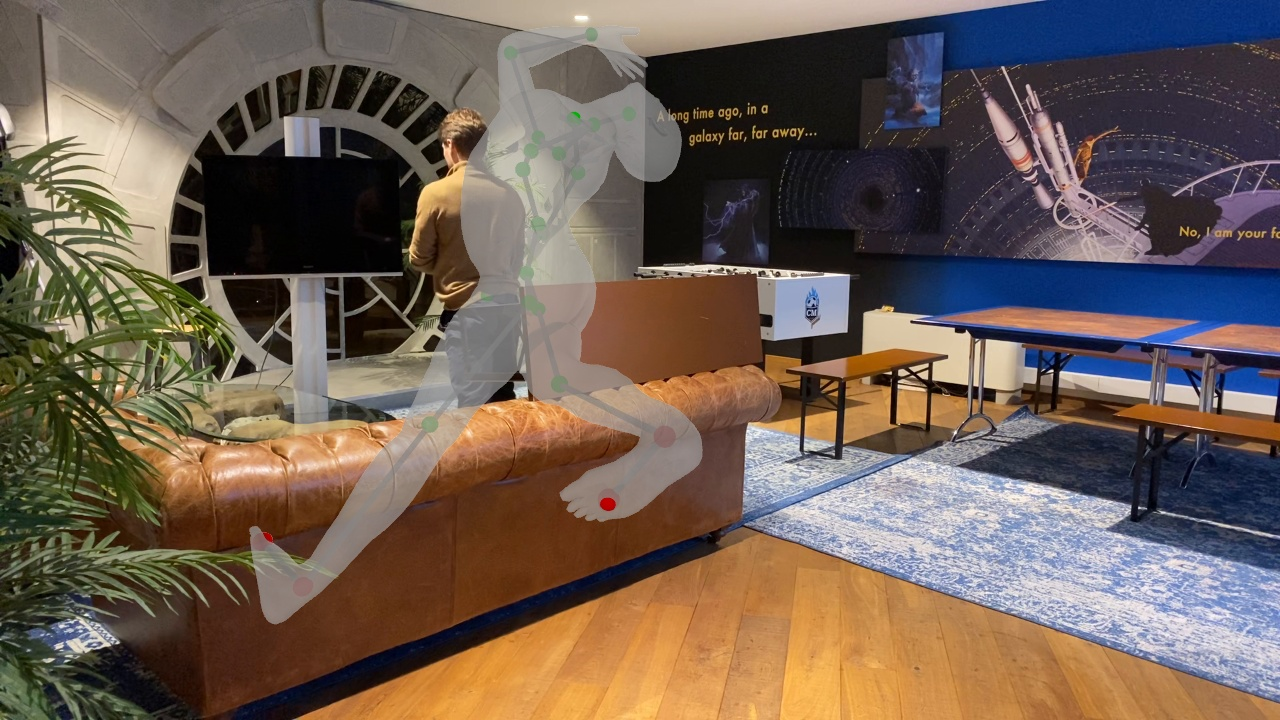
\includegraphics[width=0.3\textwidth]{Figures/humor/improvement/Rollout_stage_2/sitting_clip/rollout/frame_00000150.jpg}}
    \caption{Deviation due to rollout of Stage 2 $z$'s}
    \label{fig:humor_stage_2_rollout_deviation}
\end{figure}


With some preliminary experiments in which we began optimising $x$'s and $z$'s we found that the most successful approach to blending the decoded and optimised $x$'s was to have an L1 loss on the distance between them. We saw that when simply copying over, the propagation of small errors forward was too strong (as desribed in \figref{fig:humor_stage_2_rollout_deviation}) and the system failed to recover as the long range gradients present in the HuMoR TestOps method weren't present, and we found when blending rather than completely copying over that the weighting of the blending was another parameter that was difficult to choose, hence having a loss was the path of least resistence.

Next we experimented with jointly optimising $x$ and $z$ with a larger variety of losses. It was noted that the sitting down motion was not acheived consistenly. However as previously mentioned, the initial $z$'s encode a sitting motion, thus we conject that the $x$'s and $z$'s were fighting and this sitting motion was lost, that is to say the $z$'s move to match the $x$'s motion in which the skeleton simply clips into the floor without bending legs, thus the $z$'s begin encoding less leg bending. To avoid this issue in future experiments, the $z$'s were detached from the consistency loss making the optimised $x$'s match the decoded $x$'s.

This led us on to some experiments in which we either optimise $z$ whilst fixing $x$, or vice versa. With the $z$'s fixed at the stage 2 results, we managed to acheive a sensible sitting motion for a clip containing occluded sitting, but when we applied the same optimiser settings to a longer clip the results were no longer satisfactory. We also noted that when it did work, it required a large number of iterations, in the 1000s, which took 10mins or more, thus the speedup was not as evident as hoped (though our method would continue scaling better). In the inverse case, fixing $x$ to the final HuMoR optimised states and optimising $z$, we noted that we consistently converge in the direction of the final HuMoR $z$'s, which indicates that we are optimising in the right direction, with the best results acheived at a rollout of 5 decoding steps.

All these experiments were performed with varying numbers of decoding steps, 1, 2, 5, and 10. We found that the effect of more stable results but slower compute times with longer rollouts did manifest as intuition would suggest. 

These experiments suggest that the next direction to pursue would be an optimisation scheme in which we flip flop optimising $z$ then $x$. However considering our difficulty in achieving consistent results for the optimisation of the $x$'s with fixed $z$'s, our feeling that this might not be the optimal solution to the problem, my desire to try a new direction, and the time constraints, we deemed it time to move on and try a new method.

\subsection{Conclusion}

We found that jointly optimising the $x$'s and $z$'s did not prove an easy task to solve, which may indicate that
\begin{itemize}
    \item it is a particularly difficult problem, and therefore that the optimiser struggles to satisfy the constraints and find a good minimum for both $x$ and $z$ at the same time
    \item the coupling of the $x$'s and $z$'s in the HuMoR decoder is an important issue. We found it to be at least a minor issue as it was necessary to decouple the $z$'s from the consistency loss (matching the optimised $x$s to the decoded $x'$'s) to avoid the $z$'s being modified in such a way as to fit the unoptimised $x$'s at the beginning of the optimisation
    \item the optimiser is badly balanced
\end{itemize}
This at the very least suggests that a new decoder that does not couple $x$'s and $z$'s would be useful and worth investigating if a similar method is pursued.

In the investigations we found it possible to acheive sensible results on a given clip (for example fixing the unoptimised initial $z$'s, we can a plausible sitting motion in a small video of sitting in occlusion) but that the same settings for the optimiser failed to acheive a good result on an alternative clip. This may indicate that 
\begin{itemize}
    \item again, this is a difficult problem that the optimiser will struggle to solve
    \item the optimiser is badly balanced
\end{itemize} as before.

While many of the issues encountered may simply be due to a badly balanced optimiser, considerable effort was made to mitigate this potential issue, and therefore it is our impression that this problem is at the very least a difficult one. We have improved our intuition, fixed several issues, and understood more about the problem and our goals. We therefore can make a more informed decision with respect to which direction to pursue next. \\
We found that taking a system that was designed with autogregression in mind, and trying to parrallelise it, proved more difficult than expected. The experiments lead us to beleive that jointly optimising a sequence of poses and latent variables obtained through a single frame decoder may be a more difficult formulation of the problem than others. We therefore conclude that a method in which we model longer motion sequences may be more fruitful.

\TODO{Double check through Notes/Current\_experiments.md to see if there's anything else we can learn from the experiments}